\clearpage
\begin{flushright}
	\textit{Лекция №10}
	\textit{2015.10.13}
\end{flushright}

Речь идет о системах общего назначения.
Чтобы процесс эффективно выполнялся не должно быть страничных прерываний. Страничное прерывание – затратное действие в системе, связанное с работой менеджера памяти. 
В Unix есть страничный демон. В Windows есть что-то похожее. Страничный демон – вызывается таймером (Вызов отложенный, таймер инициирует действие. Он не может выполняться по кванту, так как будет поздно.) сканирует страницы и выгружает те страницы, к которым дольше не было обращения, чтобы, когда произойдет страничное прерывание как можно быстрее загрузить новую страницу.  
Процесс переходит с одного рабочего множества на другое. На иллюстрации (предыдущая лекция) выделяются горбики. В этот момент в памяти находятся страницы из старого и нового рабочего множества. 
Майкрософт: в их теории присутствует понятие рабочего множества. С классическим рабочим множеством это не имеет ни чего общего. Они могут заранее выделить рабочее множество. Имеется ввиду квота. Связано это с локальным и глобальным вытеснением. Процесс может держать в памяти до 10 страниц. Если процесс исчерпал свою квоту, а ему еще нужно, то он не может это сделать. В системе возникнет трешинг, т.е. резкий рост числа страничных прерываний (будет выгружать и загружать одни и те же страницы). Если возник рост кол-во страничных прерываний, то система увеличивает квоту.
Все эти исследования были в 70-х годах. У IBM было практическое доказательство рабочего множества. Процесс никогда одновременно не обращается ко всем страницам, но в процессе жизни процесс обратится к максимальному кол-ву своих страниц.

\begin{figure}[H]
    \centering
    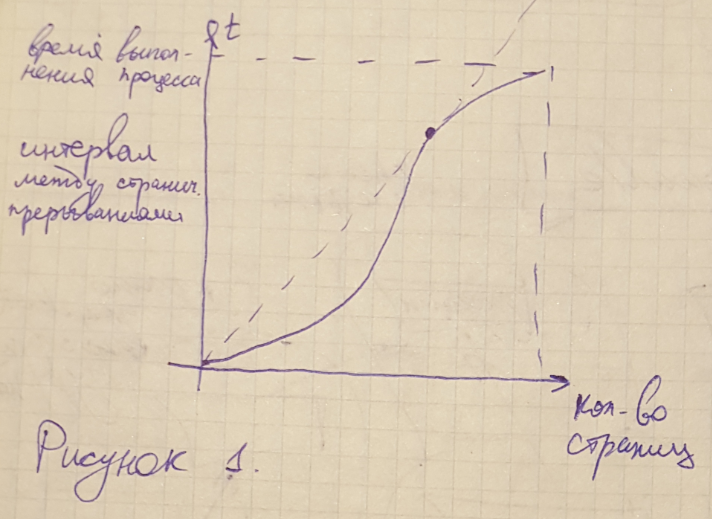
\includegraphics[width=\textwidth]{pic/1.png}
    \caption{pic}
\end{figure}

Интервал между страничными прерываниями линейно зависит от кол-ва страниц, но потом происходит перегиб. Он является следствием того, что в памяти находится все рабочее множество процесса. Эту кривую называют временем жизни.

\begin{figure}[H]
    \centering
    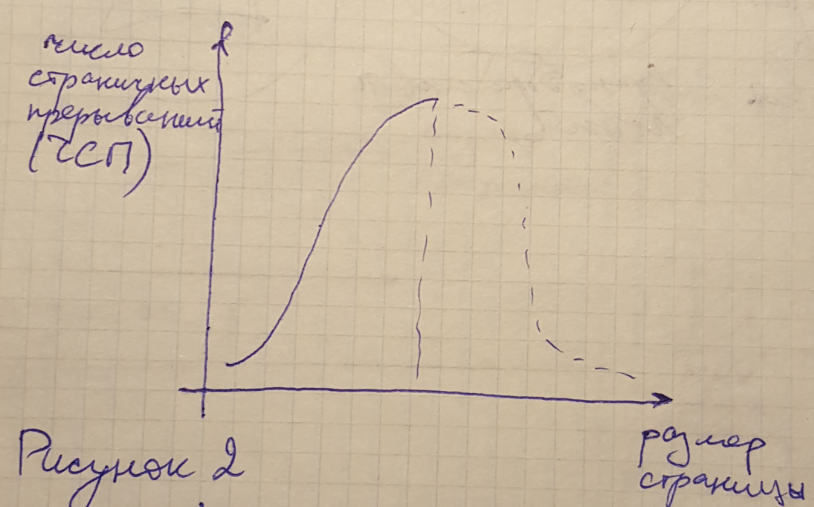
\includegraphics[width=\textwidth]{pic/2.png}
    \caption{pic}
\end{figure}

Показывает ЧСП в зависимости от размера страницы или ???. На большой странице будет выполняться меньшее кол-во команд. Наш лимит – размер программы. 

\begin{figure}[H]
    \centering
    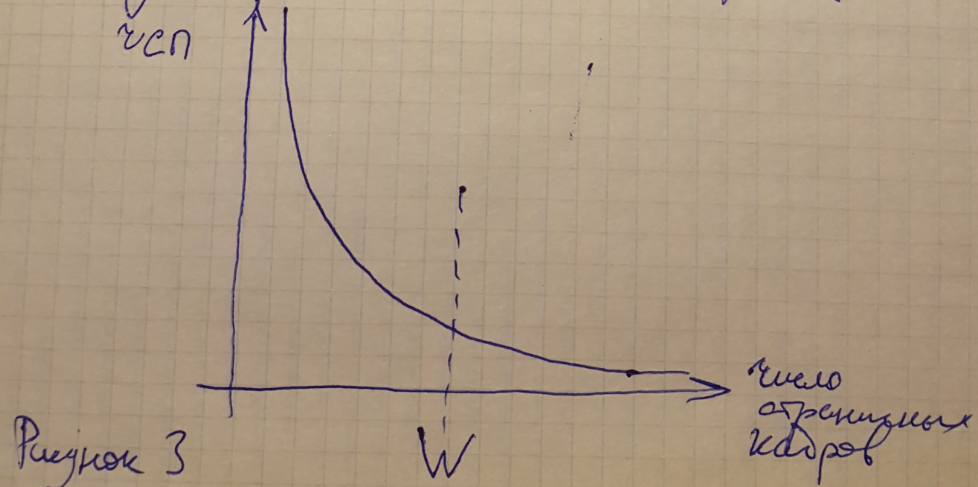
\includegraphics[width=\textwidth]{pic/3.png}
    \caption{pic}
\end{figure}

W – рабочее множество. Размер страницы фиксирован. Если квота маленькая – то ЧСП резко возрастает. 

\paragraph{Процессоры Intel}

Intel  поддерживает управление памятью сегментами по запросам (регистры GDTR – содержит начальный адрес таблицы глобальных дескрипторов ,  LDTR - содержит начальный адрес таблицы локальных дескрипторов) для страничный  CR3 – адрес где произошло страничное прерывание. PE можно отключить. Сегментное преобразование отключить нельзя. 
Для процесса выделяется один единственный дескриптор, который описывает сегмент размером 4гб. 

4гб – виртуальное адресное пространство (ВАП).

\begin{figure}[H]
    \centering
    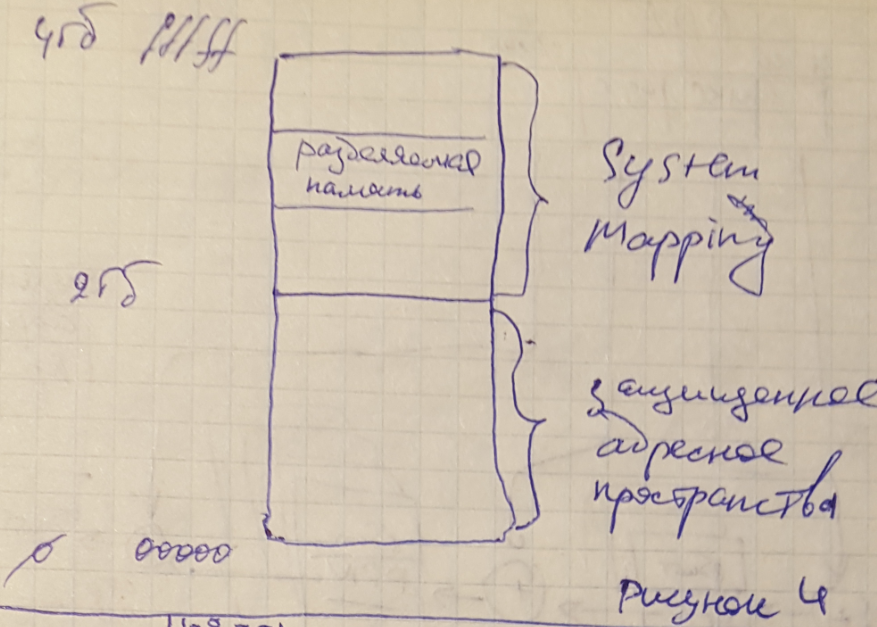
\includegraphics[width=\textwidth]{pic/4.png}
    \caption{Наиболее употребимый способ деления ВАП}
\end{figure}

Никто не копирует систему, Mapping – отображение. В ней существует область разделяемой памяти – область данных ядра системы, которая может разделяться процессами. Ни один процесс не может обратиться в адресное пространство другого процесса. Процессы взаимодействуют через адресное пространство ядра системы через системные вызовы.
Чтобы система могла работать с этими страницами, необходимо создать таблицу страниц.

\begin{figure}[H]
    \centering
    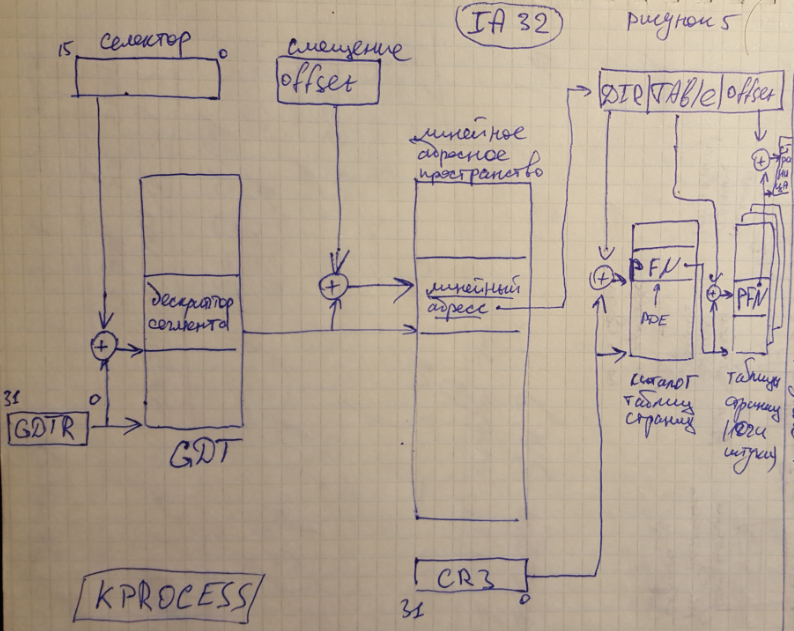
\includegraphics[width=\textwidth]{pic/5.png}
    \caption{pic}
\end{figure}

$offset$ берем из программы. Из регистров $SI$, $DI$, $BP$, $SP$.
Каждая программа имеет логическое адресное пространство. Следующее виртуальное (линейное).
Каталог таблиц страниц (КТС) содержит дескриптор таблиц. КТС один на систему и может содержать 1024 строки.
PDE - 4 байта.
PFE (page frame number) – таблица страниц. 512 таблиц на систему, 512 – на процесс. В регистре $CR3$ базовый адрес каталога таблиц страниц. Адрес (в регистре cr3) берется из дескриптора процесса.
На шине адреса будет всегда находится линейный адрес, т.е. адрес байта физической памяти. К преобразованиям шина адреса не имеет никакого отношения. 
Начиная с «пентиум про» поддерживают режим PAE (Physical AE). 
В режиме PAE виртуальный адрес делится на 4 поля.

\begin{table}[H]
\begin{tabular}{|l|l|l|l|}
\hline
31, 30 & индекс & индекс & 12 бит\\
\hline
индекс указателя на каталог страниц. & каталога страниц & таблиц страниц & смещение offset\\
\hline
\end{tabular}
\end{table}

\begin{figure}[H]
    \centering
    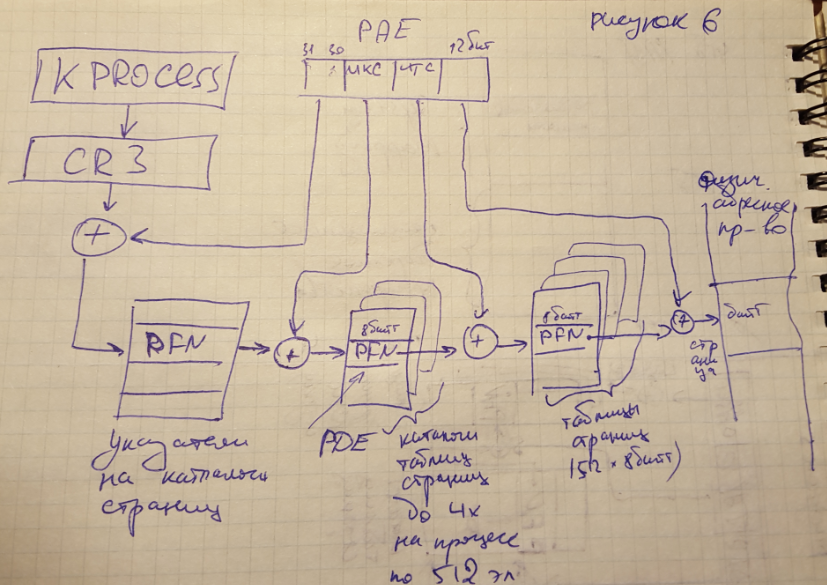
\includegraphics[width=\textwidth]{pic/6.png}
    \caption{pic}
\end{figure}

У процесса может быть 4 каталога таблиц страниц.
Существует специальная версия 32 разрядного ядра Windows с поддержкой PAE. Ядро это называется $Ntkrnipa.exe$. Кол-во преобразований больше, но обратиться можем к большей памяти. Страницы могут подгружаться. В любой системе оптимизирована загрузка страницы. Большая оперативная память позволяет держать больше программ.